% Full-paper draft v0.5 (venue unset). Center P3; P1/P2 appendix-only; elevate M1a×S join.
% Numbers: paper/evaluation_measurement_gap/EVIDENCE_MAP.md
% Wording lock: CLAIM_LEDGER.md
% Compile: pdflatex main && bibtex main && pdflatex main && pdflatex main
% Migrated to the official AAMAS 2027 template (aamas.cls, sigconf, anonymous) 2026-09-14.
\documentclass[sigconf,anonymous]{aamas}

%%% Packages not already provided by aamas.cls (which loads microtype, etoolbox,
%%% booktabs, hyperref, graphicx, xcolor, geometry, caption, float, natbib, fontenc+libertine).
\usepackage{amsmath,amssymb}
\usepackage{tikz}
\usetikzlibrary{arrows.meta,positioning,fit,calc}
\usepackage{enumitem}
\usepackage{array}

\graphicspath{{../../../out/stage4_counterfactual_analysis_final/}}

\hypersetup{colorlinks=true,linkcolor=black,citecolor=black,urlcolor=black}

\newcommand{\task}[1]{\texttt{#1}}
\newcommand{\A}{\mathcal{A}}
\newcommand{\Acap}{\mathcal{A}^{\cap}}
\newcommand{\STS}{\mathrm{STS}}
\newcommand{\Just}{\mathrm{Justifiable}}

%%% AAMAS-2027 copyright block (do not change!)
\makeatletter
\gdef\@copyrightpermission{
  \begin{minipage}{0.2\columnwidth}
   \href{https://creativecommons.org/licenses/by/4.0/}{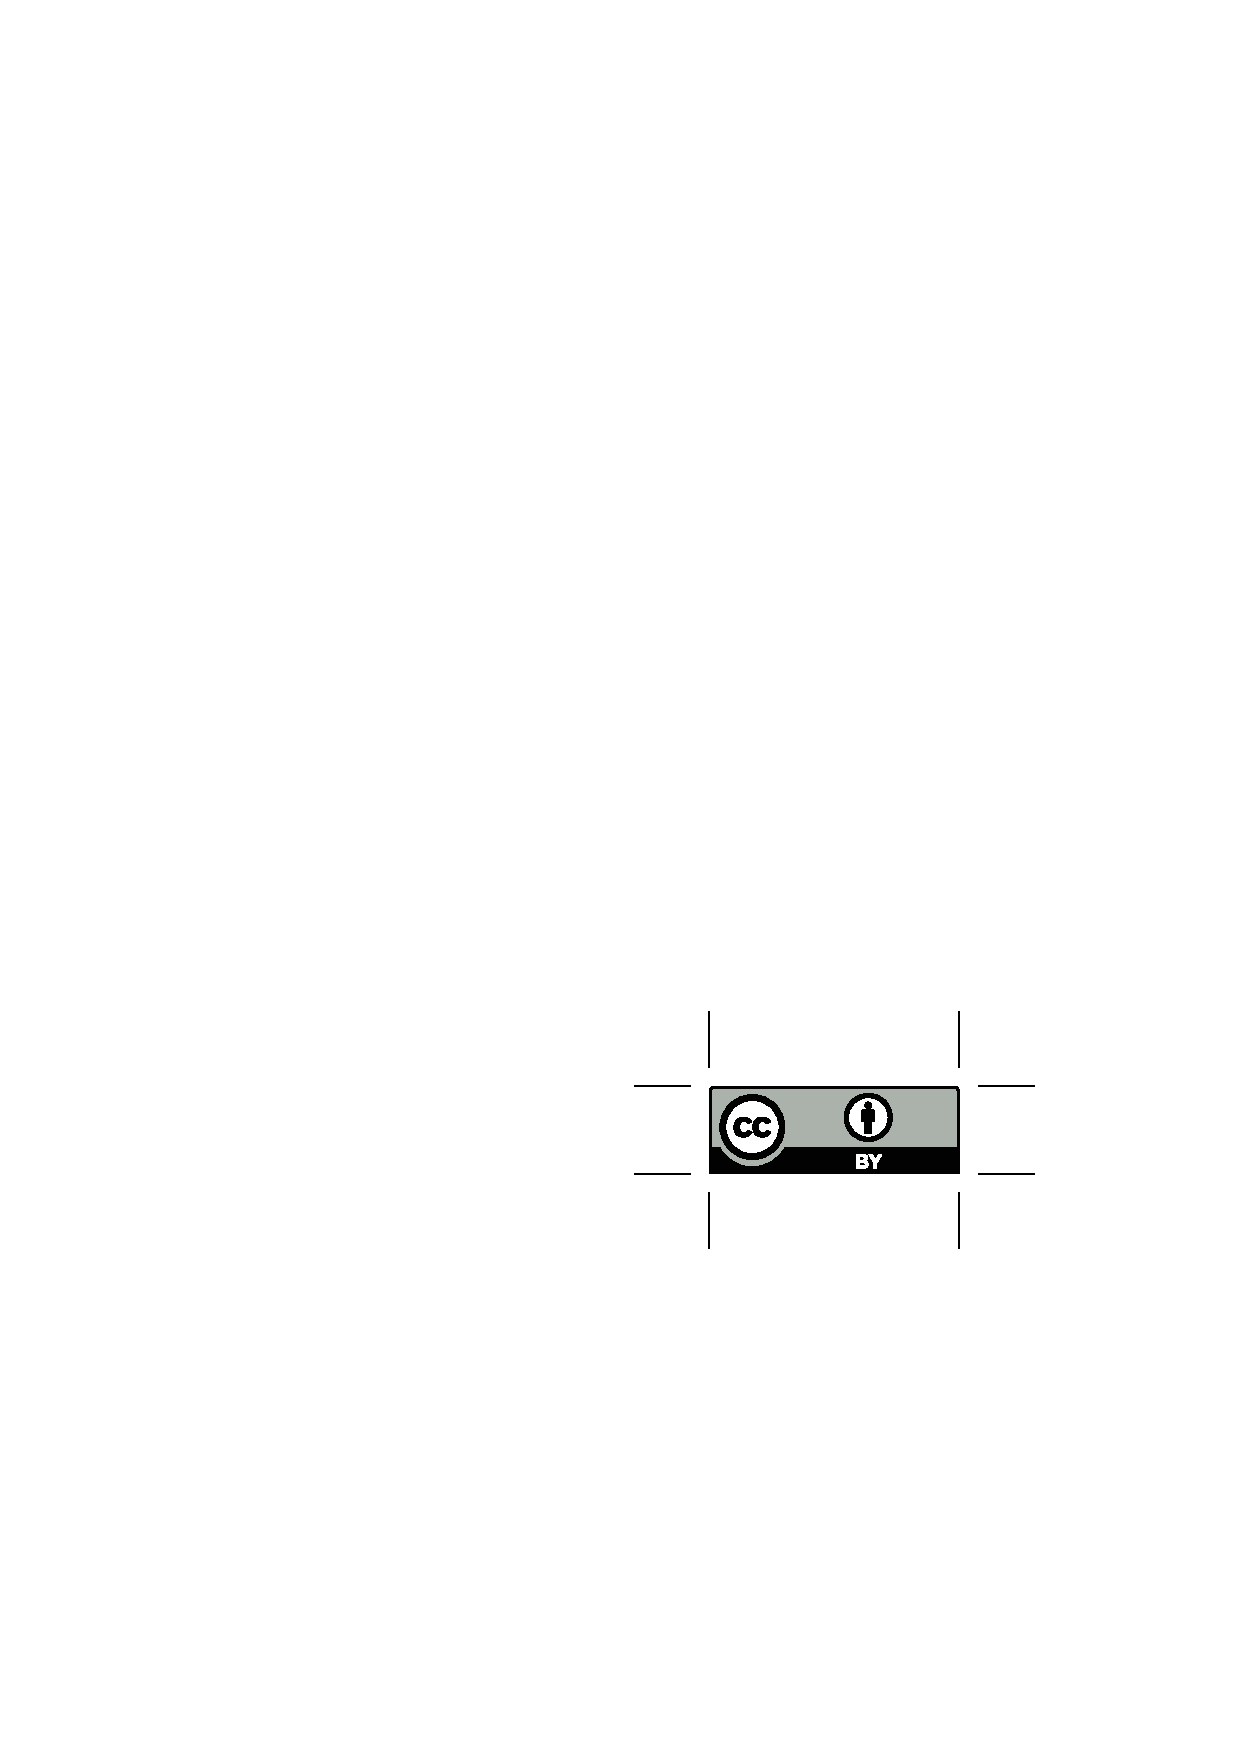
\includegraphics[width=0.90\textwidth]{by}}
  \end{minipage}\hfill
  \begin{minipage}{0.8\columnwidth}
   \href{https://creativecommons.org/licenses/by/4.0/}{This work is licensed under a Creative Commons Attribution International 4.0 License.}
  \end{minipage}
  \vspace{5pt}
}
\makeatother

\setcopyright{ifaamas}
\acmConference[AAMAS 2027]{Proc.\@ of the 26th International Conference
on Autonomous Agents and Multiagent Systems (AAMAS 2027)}{3--7 May 2027}{Hanoi, Vietnam}{M.~Baldoni, F.~Fang, W.~Yeoh, N.~Yorke-Smith (eds.)}
\copyrightyear{2027}
\acmYear{2027}
\acmDOI{}
\acmISBN{}
% TODO(vinh): fill in the OpenReview submission id once assigned.
\acmSubmissionID{}
\submissionType{Research Paper Track}

\title{From Trajectories to Evidence:\\
Auditing Observation Loss and Identifiability\\
in Computer-Use Agent Evaluation}

% TODO(vinh): authors intentionally unset (draft convention). Anonymous mode
% hides this from the typeset PDF regardless, but aamas.cls requires at least
% one \author/\affiliation/\email block to compile. Fill in for camera-ready.
\author{Anonymous Author(s)}
\affiliation{%
  \institution{Institution withheld for review}
  \country{}}
\email{}

\begin{abstract}
Computer-use-agent (CUA) reliability scores depend on how an evaluation pipeline observes a trajectory and turns that observation into evidence.
Prior CUA work already audits benchmark construction, protocol shortcuts, last-frame judges, and wrong FAIL verdicts.
This paper asks a narrower question: what happens \emph{inside} a frozen evaluator, after evidence has been collected and before a final verdict is issued?
In a locked MyPCBench trajectory-to-evidence transformation, 39 of 59 rows with recoverable gold were missed, including 13 cases in which gold had already entered the extractor's \texttt{found} set and was then discarded.
On those same legs, a locked screenshot rubric can assign a perfect score after the text channel has already discarded collected gold.
A pre-specified permissive aggregation repair released eight additional correct matches together with eighteen incorrect matches; composing all repairs was worse than leaving the extractor frozen (10 vs.\ 20 recovered rows).
Constructing an explicit last-text observation protocol then left two-sided correspondence unidentifiable in a sample of 30 HIT and 0~MISS.
We do not propose a replacement reliability metric, and we do not estimate deployed CUA reliability.
In this frozen setting, an evaluation report should make observation, evidence, abstention, and identifiability explicit before a number is read as a reliability claim.
\end{abstract}

\begin{document}
\maketitle


\section{Introduction}
\label{sec:intro}

A computer-use-agent reliability score is the output of an evaluation pipeline, not a direct observation of the episode.
That fact is established background~\citep{dong2026misscore,kane2013validating,messick1995validity}.
Leaderboards compress trajectories into binary outcomes or scalars~\citep{jang2026mypcbench,xie2024osworld,zhou2024webarena}.
The scalar is produced by a declared observation channel $I$, a parser $P$, an evidence classification $E$, a correspondence decision $Y$, and a reported score or selection $S$ (Figure~\ref{fig:gap}).

\begin{figure*}[t]
\centering
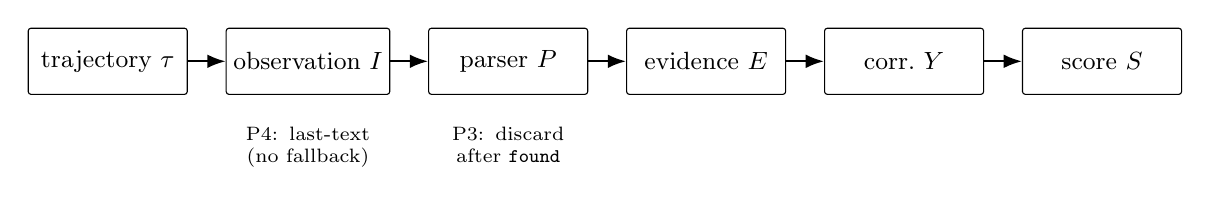
\begin{tikzpicture}[
  font=\small,
  box/.style={draw, rounded corners=1pt, align=center, inner sep=2.6pt,
              minimum height=8.4mm, minimum width=2.02cm},
  arr/.style={-{Latex}, thick},
  lab/.style={font=\scriptsize, align=center, text width=2.02cm}
]
\node[box] (tau) {trajectory $\tau$};
\node[box, right=4.8mm of tau] (I) {observation $I$};
\node[box, right=4.8mm of I] (P) {parser $P$};
\node[box, right=4.8mm of P] (E) {evidence $E$};
\node[box, right=4.8mm of E] (Y) {corr.\ $Y$};
\node[box, right=4.8mm of Y] (S) {score $S$};
\draw[arr] (tau) -- (I);
\draw[arr] (I) -- (P);
\draw[arr] (P) -- (E);
\draw[arr] (E) -- (Y);
\draw[arr] (Y) -- (S);
\node[lab, below=2.8mm of I] {P4: last-text\\(no fallback)};
\node[lab, below=2.8mm of P] {P3: discard\\after \texttt{found}};
\end{tikzpicture}
\caption{A reliability score is constructed along $\tau\to I\to P\to E\to Y\to S$.
The empirical core (Section~\ref{sec:s3}) is discard \emph{after} gold has entered the parser's accumulator.
The constructive sequence (Section~\ref{sec:p4}) makes $I$ explicit and records where two-sided correspondence remains unidentifiable.
Three analytic labels---outcome, observation, justification---organize that evidence; they are not proposed as new laws of measurement.}
\label{fig:gap}
\end{figure*}

Existing work has already shown that those pipelines can fail.
Dong et al.\ treat a CUA score as a pipeline output and find that public FAIL verdicts can be wrong~\citep{dong2026misscore}.
Shao et al.\ show that agent-benchmark scores support capability claims only when the protocol keeps the intended capability necessary for success~\citep{shao2026protocolvalidity}.
Xue et al.\ and Rosset et al.\ document last-frame and overloaded-trajectory observation loss in visual web judging~\citep{xue2025illusion,rosset2026verifiers}.
Bean et al.\ give an operational construct-validity checklist for LLM benchmarks~\citep{bean2025measuring}.

The remaining question is narrower.
What happens when the evaluation \emph{instrument} itself is frozen and treated as the experimental object---not the agent, and not the published verdict?
In particular, what happens \emph{inside} a frozen observation-to-evidence transformation, after evidence has been collected and before a final PASS/FAIL is issued?

In this frozen MyPCBench extractor, determining gold was present in the trajectory and had already entered the intermediate \texttt{found} set, but fail-closed aggregation discarded it before the correspondence decision.
Of 59 rows with recoverable gold, 39 were missed; 13 of those 39 misses are this post-collection discard.
On those 13 rows, a locked screenshot rubric can still report $S=100$ after the text channel has discarded collected gold.
A pre-specified permissive aggregation repair then released eight additional correct matches together with eighteen incorrect matches.
Permissiveness did not restore the intended measurement.

We then asked what happens if observation and identifiability are made explicit rather than left implicit in an existing extractor.
Under a declared last-text channel with no screenshot or tool-trace fallback, completion need not yield determining evidence, interface compliance need not identify a two-sided estimand, and a competent sample of 30 HIT and 0~MISS left two-sided correspondence unidentifiable under the pre-locked rule.

This is an instrument-level audit of a frozen CUA evaluator, with a constructive check on what an explicit observation protocol can still fail to identify.
It is not a general theory of CUA reliability, not a replacement metric, and not a claim that existing public benchmarks are invalid.

\section{Background and related work}
\label{sec:rw}

\subsection{CUA and agent evaluation}
\label{sec:rw-cua}

Desktop and web CUAs are scored in OSWorld, WebArena, VisualWebArena, and MyPCBench~\citep{xie2024osworld,zhou2024webarena,koh2024visualwebarena,jang2026mypcbench}.
WebArena-Verified re-audits web tasks toward deterministic, offline evaluators~\citep{hattami2025webarena}.
Tool-using and interactive-coding agents are scored by state match, multi-trial reliability, and collateral-damage tests~\citep{yao2025taubench,trivedi2024appworld}.

Shao et al.\ audit 2{,}385 traces across 15 benchmarks for exposure, exploitation, and score inflation~\citep{shao2026protocolvalidity}.
That is protocol validity: shortcuts and invalid scoring paths.
This paper does not rest on the claim that ``scores justify claims,'' which Shao already makes.
It asks a different grain: once a protocol is frozen, what evidence does its observation channel recover, and can that evidence identify the correspondence claim one wanted to make?

\subsection{Validity and measurement}
\label{sec:rw-validity}

We do not invent validity theory.
Messick treats validity as scientific inquiry into score meaning and use~\citep{messick1995validity}.
Cronbach and Meehl locate construct validity in the network of inferences around a test~\citep{cronbach1955construct}.
Kane's argument-based approach is the principle we rely on: it is the proposed interpretations and uses of scores that are validated, not the scores themselves~\citep{kane1992argument,kane2013validating}.
Jacobs and Wallach import measurement modeling into computational systems~\citep{jacobs2021measurement}.
Raji et al., Bowman and Dahl, and Bean et al.\ diagnose construct-validity and benchmarking failures when a finite task is treated as a general capability measure~\citep{raji2021everything,bowman2021fix,bean2025measuring}.

What this paper adds is not a new validity framework.
It is an instrument-level audit at the trajectory--observation--evidence grain, under a frozen protocol, with an isolation of post-collection discard and a signed repair experiment.

\subsection{Evaluator and observation audits}
\label{sec:rw-audit}

Dong et al.\ is the closest CUA paper and must be confronted directly~\citep{dong2026misscore}.
They state that a score is the output of a pipeline in which tasks can be stale, trajectories can omit decisive visual evidence, evaluators can reject valid alternatives, and aggregate reports can hide the cause of failure.
They then retrospectively audit 150 public \emph{failure-scored} trajectories from five benchmarks and find that 15.3\% of FAIL verdicts are wrong (10.7\% evaluator false negatives; 4.7\% broken tasks), with a further 3.3\% unclear from the released evidence.
That is a verdict audit: is the published FAIL correct?

Xue et al.\ (Online-Mind2Web / WebJudge) show that last-frame and underspecified LLM judges mis-score web agents and propose preserving critical intermediate screenshots~\citep{xue2025illusion}.
Rosset et al.\ argue that last-frame and overloaded full-trajectory judges both fail, and build a verifier that selects diagnostic screenshots per rubric criterion~\citep{rosset2026verifiers}.
Those papers establish last-frame observation loss as a known failure of \emph{visual} CUA judging.
They do not freeze a last-text typed extractor and measure discard after gold has already entered an accumulator.

WeaveBench reports that outcome-only grading overestimates pass rate relative to a trajectory-aware judge~\citep{li2026weavebench}.
L\`u et al.\ make automatic trajectory judges themselves the object of evaluation~\citep{lu2025agentrewardbench}.
Cao et al.\ document procedure-aware ``corrupt success''; Advani documents false success as confident closure without the implied outcome~\citep{cao2026corruptsuccess,advani2026falsesuccess}.

\subsection{Positioning}
\label{sec:rw-pos}

Dong audits \emph{verdicts} on public traces.
We audit a \emph{frozen transformation} $I\to P\to E$ on trajectories we already hold, then construct an observation-grounded measurement and record where construction stops.

\begin{quote}
Dong: retrospective verdict audit over public CUA traces, focused on whether released FAIL verdicts are correct.\\[4pt]
This paper: treats the evaluation instrument as the experimental object, freezes the observation/evidence transformation, audits evidence loss inside that transformation (including gold collected then discarded), experimentally tests permissive repairs, and records identifiability boundaries encountered when constructing an observation-grounded last-text measurement.
\end{quote}

Shao's axis is exposure $\to$ exploitation $\to$ misleading shortcuts.
Ours is observation $\to$ evidence $\to$ correspondence, including measurement loss after evidence has become available.
Neither axis subsumes the other.

A neighboring literature localizes \emph{agent} failures to a responsible component or step~\citep{zhang2025whoandwhen}.
That is not this paper's object.
We audit the evaluation instrument's observation channel, not which agent action caused the task to fail.

\section{The instrument as the object of analysis}
\label{sec:measurement}

Equation~\eqref{eq:pipe} is the object of analysis, not a newly discovered law:
\begin{equation}
\tau \;\longrightarrow\; I \;\longrightarrow\; P \;\longrightarrow\; E \;\longrightarrow\; Y \;\longrightarrow\; S.
\label{eq:pipe}
\end{equation}
$I$ is the declared observation channel.
In the constructive studies of Section~\ref{sec:p4}, $I$ is last assistant text, never screenshots or tool traces as a silent fallback.
That channel is a declared severe protocol, not a claim that last-text is canonical for CUA evaluation.
$P$ recovers at most one unique candidate span, or none.
$E$ is DETERMINING iff that span parses as specification-kind $k$, not iff it equals $\mathrm{value}(L)$.
$Y$ is HIT/MISS only when $E$ is DETERMINING and $L$ is independent of this episode's answer.
ABSTAIN is missing correspondence measurement, not task failure.
$S$ is any scalar or selection computed from $Y$, or from a coarser rubric that never exposes $Y$.

Three analytic categories organize the evidence below.
They are not a new ontology, and they overlap Dong's construction / observation / scoring / reporting stages~\citep{dong2026misscore}:
\begin{itemize}[leftmargin=1.4em,itemsep=2pt]
\item \textbf{Outcome gap:} $S$ need not correspond to independently measured world tracking.
\item \textbf{Observation gap:} evidence in $\tau$ need not enter $I$ or survive $P$.
\item \textbf{Justification gap:} recovered evidence need not identify the reliability claim one wanted to make (including two-sided correspondence).
\end{itemize}
We use the labels because they match the grain of the audit.
Where ``measurement gap'' would be read as a contribution of measurement theory, we mean only this local mismatch among score, observation, and justified claim under a declared protocol.

As formal bookkeeping, write
\begin{multline}
\mathcal{M}(\tau,\mathcal{I})
=\{\,C:\ \text{the evidence $C$ requires}\\
\text{is recoverable under $I$}\\
\text{and the inference is non-circular}\,\}
\label{eq:M}
\end{multline}
for the set of reliability claims justified under a declared observation protocol.
$\mathrm{Observable}_{\tau}(\tau)$ need not equal $\mathrm{Observable}_{I}(\tau)$: a typed fragment can exist in the trajectory and still be missed by the instrument.
\[
\neg \Just(C\mid \tau,I) \;\neq\; \mathrm{False}(C).
\]
If the pipeline cannot recover the evidence a claim requires, the claim is unjustified \emph{from this measurement}; that is not a demonstration that the agent failed.
$\mathcal{M}$ is not a reliability metric, not a new validity theory, not a theorem of reliability, and not empirically validated.
Typed correspondence---$Y=\mathrm{HIT}$ implies a kind-parse matching $L$---is a specification-level implication of the declared HIT rule under no-leakage maps, not a proof.

Table~\ref{tab:map} is the evidence map.
There is one core empirical result.
Two supporting checks on the same MyPCBench family---that a reported score can dissociate from independently measured tracking, and that evaluation can empty a comparison---are in Appendix~\ref{app:s1} and Appendix~\ref{app:s2}.
They are not the contribution.

\begin{table}[H]
\centering
\caption{Evidence map. Populations are not added. This is not a prevalence table.}
\label{tab:map}
\small
\begin{tabular}{@{}llp{0.58\columnwidth}@{}}
\toprule
Role & Source & Licensed reading \\
\midrule
Core & P3 & Post-collection discard (M1a) and signed repair non-dominance in one frozen extractor \\
Secondary & P4 & Constructive observation/identifiability boundaries, especially Form$\neq$two-sided ID and a HIT-only sample \\
Supporting & P1, P2 & Appendix only: score need not track the world; evaluation can change the evidential basis of a comparison \\
Supporting & Path A & Released FAIL mixes empty $I$ (126) and mismatch (173) on an admitted string/URL slice; not an unjustified-FAIL rate \\
Formal & $\mathcal{M}(\tau,\mathcal{I})$ & Bookkeeping for claims justified under a declared $I$ \\
Consequence & Table~\ref{tab:slots} & Eight reporting questions; not a validated standard \\
\bottomrule
\end{tabular}
\end{table}

\section{Evidence loss inside a frozen extractor}
\label{sec:s3}

This section is the empirical core.
We freeze the evaluator and inspect the maps that turn a trajectory into a reported value.
The contribution is not that missing evidence matters in general---Dong, Xue, and Rosset already document observation and evaluator failures~\citep{dong2026misscore,xue2025illusion,rosset2026verifiers}.
The contribution is isolating a mechanism \emph{inside a frozen trajectory-to-evidence transformation} and testing whether permissive repair restores the intended measurement.

The unit is a row: one component of the determining set on one leg (134 rows over 57 legs).
A row is R1-positive if the gold value is literally present in the agent's answer ($n=59$: 20 MATCH + 39 RECALL\_MISS).
The remaining 61 rows are ABSENT.
Rates below are conditional on these audited sets.
They are not a false-negative rate of the agent, not an evaluator-disagreement rate, and not a screenshot-omission rate.

The frozen instrument recovers 20 of 59 R1-positive rows (sensitivity $0.339$) and misses 39 (Table~\ref{tab:causes}).

\begin{table}[H]
\centering
\caption{Cause of the 39 recall misses. Meanings are locked. Frozen extractor \texttt{3242c30}.}
\label{tab:causes}
\small
\begin{tabular}{lrl}
\toprule
Cause & $n$ & Meaning \\
\midrule
M1a & 13 & gold entered \texttt{found} and was discarded \\
M1b &  7 & candidates disagree; gold is not among them \\
M2  &  9 & no label hit anywhere in the answer \\
M3  &  5 & label hit; gold outside every $\pm$window \\
M4  &  5 & instrument reported a non-gold value \\
\bottomrule
\end{tabular}
\end{table}

\paragraph{Post-collection discard.}
In this frozen extractor, we isolate a post-collection discard mechanism: determining gold was present in the trajectory and had entered the intermediate \texttt{found} set, but was removed by fail-closed aggregation before the final correspondence decision.
That location is not visible to a verdict-level audit that only observes final PASS/FAIL judgments.

In 13 of 39 misses the extractor had already accumulated the gold value and fail-closed aggregation discarded it.
In 7 of those 13, gold was a strict majority of the accumulated candidates.
This is not agent failure: the gold string was in the answer and in the accumulator.
It is not generic missing data: the observation existed at an intermediate instrument state.
It is not last-frame screenshot omission: the channel is text.
It is not ordinary judge error: no LLM judge sits in this extractor.
On the same 13 rows, a locked screenshot-rubric $S$ can be 100 while typed gold had already been collected and discarded: 7 of 10 joinable rows have $S=100$ (3 rows have no locked per-leg $S$ and are not imputed); all 9 M1a rows that sit in $\A$ have pair-level $Y=0$ (Table~\ref{tab:m1a-s100}; row-level detail in Appendix~\ref{app:m1a-join}).
The gold string also appears in recorded action/response text \emph{before} the final answer on 8 of 13 rows.
That is not evidence that a screenshot contained gold, and it is not a 171-trajectory audit.
It is the local ``why care'' on this instrument: a full-trajectory visual rubric can look like success on the same episode whose typed evidence did not survive the extractor.

\begin{table}[H]
\centering
\caption{Locked screenshot-rubric $S$ on the 13 M1a rows. Not a prevalence estimate.}
\label{tab:m1a-s100}
\small
\begin{tabular}{lr}
\toprule
Quantity & $n$ \\
\midrule
Joinable locked $S$ & 10/13 \\
$S=100$ among joinable & 7/10 \\
In $\A$ with pair $Y=0$ & 9/9 \\
Gold in earlier traj.\ text & 8/13 \\
\bottomrule
\end{tabular}
\end{table}

M1 is not exclusive to misses (25 of 61 ABSENT rows are also M1); M1a is the cause that names recoverable-but-discarded evidence.
No single-cause story is licensed.
A pre-registered secondary prediction that misses would concentrate on injected-world tasks \emph{failed} (confidence intervals overlap; we do not replace it with a reversal).

\paragraph{Permissive repair is not guaranteed to restore the measurement.}
Four layer interventions were specified before the run.
R-AGG (plurality) targets M1a; R-SCOPE, R-CMP, and R-CHAN target other miss classes; ALL composes them.
No configuration is offered as a replacement instrument.
Table~\ref{tab:repairs} reports the signed outcome that bears on the contribution; the full six-configuration diagnostic is in Appendix~\ref{app:s3}.

\begin{table}[H]
\centering
\caption{Signed repair outcome on the frozen extractor. Sensitivity is over 59 R1-positive rows. Full configurations: Appendix~\ref{app:s3}.}
\label{tab:repairs}
\footnotesize
\setlength{\tabcolsep}{3pt}
\begin{tabular}{lrrr}
\toprule
Config & Sens./59 & Signed change vs.\ frozen & MATCH destroyed /20 \\
\midrule
FROZEN & 20 & --- & 0 \\
R-AGG  & 28 & $+8$ correct, $+18$ wrong & 0 \\
ALL    & 10 & worse than frozen & 16 \\
\bottomrule
\end{tabular}
\end{table}

Under the pre-specified permissive aggregation repair, 8 additional correct matches were released together with 18 incorrect matches.
R-AGG is the only intervention that raises sensitivity ($20\to 28$); it does so by releasing 26 abstentions.
Recovering more evidence is not equivalent to recovering the intended measurement.
The result is not a general theorem about parsers; it shows that permissiveness did not restore the intended measurement in this frozen instrument.
Composing all repairs was worse than leaving the extractor frozen (10 vs.\ 20).
A later-layer comparison repair cannot recover an upstream miss (R-CMP is bit-identical to FROZEN; Appendix~\ref{app:s3}).

The licensed claim is instrument-specific.
We do not estimate how often M1a occurs in other CUA evaluators, and we do not ship R-AGG as a method.

\section{Constructive boundaries of observation-grounded evaluation}
\label{sec:p4}

Section~\ref{sec:s3} shows that an existing instrument can lose evidence \emph{after} collection.
This section asks what happens if we explicitly construct an observation-grounded protocol rather than auditing an inherited extractor.

P4 is not four failed metrics, not a leaderboard, not a replacement reliability metric, and not an evaluation of Flash's reliability.
It is one constructive sequence showing successive boundaries: empty observation, then interface compliance without two-sided identifiability, then dense HIT-only observation without two-sided variation (Table~\ref{tab:p4seq}).
The channel remains last assistant text, with no screenshot or tool-trace fallback.
Execution status is never HIT/MISS.
ABSTAIN is missing correspondence measurement, not task failure.

\begin{table}[H]
\centering
\caption{Constructive boundaries under a declared last-text channel. Not a ranking of agents and not four failed metrics.}
\label{tab:p4seq}
\small
\begin{tabular}{@{}>{\raggedright\arraybackslash}p{0.30\columnwidth}
                   >{\raggedright\arraybackslash}p{0.34\columnwidth}
                   >{\raggedright\arraybackslash}p{0.28\columnwidth}@{}}
\toprule
Boundary & Locked observation & Licensed reading \\
\midrule
Determining $E$ absent from declared $I$ & 40/40 \texttt{DONE}; 30 ABSTAIN; Flash Cov.\ $0.1667$ & Completion $\neq$ evidence in $I$ \\
Form $\neq$ two-sided ID & Form $0.9333$; H3 N/E & Interface $\neq$ two-sided estimand \\
HIT-only sample, locked rule & 30 HIT / 0 MISS; $I_{CC}=0$; G2 10/10 & Two-sided CC unidentified here \\
\bottomrule
\end{tabular}
\end{table}

\subsection{Evidence can be absent from the declared channel}
\label{sec:p4bc}

P4-B scores last-text HIT/MISS/ABSTAIN on 40 confirmatory episodes ($N_B=20$ clusters $\times$ two models).
All 40 legs terminated \texttt{DONE}.
The instrument returned HIT~5, MISS~5, ABSTAIN~30.
Every abstention is \texttt{no\_anchor}: no instruction-anchor substring on a newline-terminated line of last text.
The instrument did not then mine screenshots, tools, or intermediate turns.

P4-C scores unstructured last text against independent gold (metric v1).
Flash confirmatory $N_C=30$: HIT~3, MISS~2, ABSTAIN~25; coverage $0.1667$.
Coverage fails its pre-specified gate ($\ge 0.5$).

These two stages are one lesson.
Natural agents need not communicate determining evidence through an undeclared last-text channel, and terminal completion is not observation-grounded measurement success.
The result is not that last-text is the right CUA channel, and not that the agent is incompetent.
It is that if the declared channel does not contain determining evidence, the instrument must abstain rather than silently fall back.

\subsection{Interface compliance does not imply two-sided identifiability}
\label{sec:p4c2}

Metric v2 requires a declared \texttt{CLAIM:} line---an interface constraint, not itself evidence.
Flash $N=30$: HIT~26, MISS~2, ABSTAIN~1, unscored~1; Form $0.9333$ (gate pass).
Ordinary MISS exists (two clusters).
The C2-intended discrimination floor is NOT\_EVALUABLE (8 eligible $<10$; miss rate $0$ on that slice).
Interface compliance can pass while two-sided correspondence remains unevaluable.
Form is not validity.

\subsection{A competent sample can still lack negative variation}
\label{sec:p4d}

The question was observability of two-sided correspondence without a MISS quota.
Flash $N=30$: HIT~30, MISS~0, ABSTAIN~0; Form $1.0000$; $I_{CC}=0$ under the locked rule ($I_{CC}=1$ iff at least 8 HIT and 8 MISS).
Plus-competence held (G2: 10/10 HIT).
Minus and plus-minus slices: 10/10 HIT each.
Classification: W1---challenge weak / correspondence remains unobservable.
The failing gate is G3.

Under the pre-locked rule, this sample did not contain enough negative observations to identify the two-sided estimand.
$I_{CC}=0$ is a protocol-and-sample observability result.
It is not a finding that competence causes unidentifiability, not a finding that the agent is unreliable, and not a claim that Flash is perfectly reliable.
The workstream is closed: distractors are not amped, the parser is not retuned, and a MISS factory is not introduced.

\section{Discussion}
\label{sec:discuss}

\paragraph{What P3 establishes.}
In this frozen extractor, evidence can be collected and then discarded.
Gold entered \texttt{found} and fail-closed aggregation removed it before $Y$.
A verdict-level audit that sees only PASS/FAIL cannot locate that step.

\paragraph{Why repair is not enough.}
Under the pre-specified permissive aggregation repair, eight additional correct matches were released together with eighteen incorrect matches.
Composing all repairs was worse than the frozen extractor.
Permissiveness is not, in this instrument, a measurement repair.

\paragraph{What P4 adds.}
Making observation explicit does not automatically make two-sided correspondence identifiable.
A declared last-text channel can be empty of determining evidence; a passing Form score can leave the two-sided estimand unevaluable; a HIT-only sample can leave $I_{CC}=0$ under a rule that requires negative observations.
P4 is subordinate to P3: it bounds what construction can still fail to identify, rather than offering a replacement score.

\paragraph{Public last-answer oracles collapse two FAILs.}
On 299 released FAIL from the admitted WebArena / VisualWebArena string and URL slice (ELIGIBLE episodes; trajectories from L\`u et al.~\citep{lu2025agentrewardbench}), the oracle records a single FAIL for two different observation states: 126 trajectories have no checkable candidate in the declared last-answer / last-URL channel $I$, and 173 have a candidate that then fails to match gold (Appendix~\ref{app:patha}).
ABSTAIN $\neq$ MISS.
$V{=}0$ does not say which.
Empty $I$ yielding FAIL is the spec-correct behaviour of \texttt{string\_match}/\texttt{url\_match}; it is not a demonstration that those 126 FAIL verdicts are unjustified from $I$, and it is not Dong's human review of incorrect FAIL.
We do not report an AgentRewardBench-wide rate.

\paragraph{What we do not establish.}
We do not claim that CUA evaluators fail, that public benchmarks are invalid, that last-text is canonical, that Flash is reliable or unreliable, that $\mathcal{M}(\tau,\mathcal{I})$ is a validated theory, or that a new reliability metric has been produced.
The object of evaluation, in this paper, is what a frozen protocol can justify---not which agent scores highest.

\section{A practical reporting consequence}
\label{sec:framework}

Table~\ref{tab:slots} lists eight questions that follow from the analysis.
These eight questions are a practical reporting consequence of the analysis, not a validated universal standard.
They are not a new metric and not a theorem.

\begin{table}[H]
\centering
\caption{Eight reporting questions for a CUA reliability number in a frozen evaluation setting.}
\label{tab:slots}
\small
\begin{tabular}{|p{0.22\columnwidth}|p{0.70\columnwidth}|}
\hline
\textbf{1. Target} & Reliability of what system, on what task family, for what use? \\
\hline
\textbf{2. Measurand} & What independently defined state or outcome is correctness? Who locked $L$? \\
\hline
\textbf{3. Observation} & What part of $\tau$ is actually observed ($I$)? What is forbidden as silent fallback? \\
\hline
\textbf{4. Evidence} & What makes an observation DETERMINING? What is NONDETERMINING? \\
\hline
\textbf{5. Correspondence} & How is evidence matched to the measurand? Is the matcher allowed to see $\mathrm{value}(L)$? \\
\hline
\textbf{6. Abstention} & What happens when evidence is insufficient? Is ABSTAIN distinct from MISS and from execution failure? \\
\hline
\textbf{7. Non-leakage} & Can the procedure see the answer it is supposed to evaluate? \\
\hline
\textbf{8. Identifiability} & Does the sample contain enough positive \emph{and} negative variation to support the intended claim (one-sided vs.\ two-sided)? \\
\hline
\end{tabular}
\end{table}

\section{Limitations}
\label{sec:limits}

M1a is instrument-specific until transported; we did not transport it.
Studies~1--3 share a MyPCBench family; populations are not added, and the result is not a multi-benchmark prevalence estimate.
P4 is a constructed slate, not a public benchmark.
Last-text $I$ is a declared severe observation channel, not a canonical CUA protocol; Xue and Rosset already show that visual last-frame judging is itself lossy~\citep{xue2025illusion,rosset2026verifiers}.
P4-D is a protocol-and-sample identifiability result ($I_{CC}=0$ because the sample has 0~MISS under a rule that requires both sides), not a reliability estimate for Flash.
$\mathcal{M}(\tau,\mathcal{I})$ is bookkeeping with no empirical implementation.
The paper does not measure deployed CUA reliability or safety.
Path~A does not use human success as correspondence gold and does not claim that empty last-answer FAIL is an incorrect oracle verdict.

We also audited public CUA artifacts for an independently specified evaluator exposing an intermediate evidence state at a grain suitable for testing post-collection discard.
No corpus satisfied the frozen eligibility contract without changing the observation protocol or evaluator.
We therefore do not claim transport of M1a beyond the frozen MyPCBench instrument.

\section{Conclusion}
\label{sec:conc}

A frozen CUA evaluation instrument can discard collected gold after it has entered an intermediate evidence set.
A pre-specified permissive repair can worsen correspondence, releasing more wrong matches than correct ones.
Constructive observation protocols then expose identifiability limits: even an explicit channel can leave two-sided correspondence unidentified when the sample has no negative variation.
Evaluation reports should therefore expose the evidential basis of a reliability claim---observation, evidence, abstention, and identifiability---before the number is interpreted.

\bibliographystyle{ACM-Reference-Format}
\bibliography{refs}

\clearpage
\appendix
\section{Study 1 details}
\label{app:s1}

Study~1 is an existence / dissociation demonstration, not a prevalence estimate.
The frozen schedule executed 46 of 50 intended cells (92 legs).
35 legs are execution failures; 24 pairs are valid.
Primary lanes are reported separately (Table~\ref{tab:s1}).
A size ablation and an exploratory Flash lane exist and are not pooled.
We do not headline a pooled invariance rate.

\begin{table}[H]
\centering
\caption{Study~1 primary lanes (existence sample). Invariance is Type~A over tracking-valid pairs. Intervals are Clopper--Pearson 95\% and are wide. Source: Stage-4 snapshot \texttt{b7b4203}.}
\label{tab:s1}
\small
\begin{tabular}{lrrrrr}
\toprule
Lane & Valid & Track-valid & Type~A & Sens.\ & Type~B \\
\midrule
Claude          & 9 & 7 & 6 & 1 & 2 \\
GPT-5.5         & 8 & 7 & 3 & 4 & 1 \\
Qwen3.5-35B-A3B & 1 & 1 & 1 & 0 & 0 \\
\bottomrule
\end{tabular}
\end{table}

Claude: invariance $6/7=0.857$ ($[0.421,0.996]$).
GPT-5.5: $3/7=0.429$ ($[0.099,0.816]$).
Qwen3.5-35B-A3B: one valid pair, Type~A ($[0.025,1.000]$).
Paired world interventions follow a counterfactual design~\citep{pearl2009causality}; they are a method for this dissociation, not the paper's main contribution.

\begin{figure}[H]
\centering

\includegraphics[width=0.98\columnwidth]{score_pairs_primary.png}
\caption{Study~1 primary lanes: paired base vs.\ counterfactual scores on valid pairs. Ablation and exploratory lanes are not pooled into Table~\ref{tab:s1}.}
\label{fig:s1pairs}
\end{figure}

\section{Study 2 details}
\label{app:s2}

Locked heading: evaluation and selection can change the evidential basis of a reliability comparison.
It is not a claim that the evaluator changes the truth.

Three agents each ran a pre-registered schedule of 57 legs: GPT-5.5, Qwen3.8-Flash, and Claude Opus~4.6 (Table~\ref{tab:coverage}).
The inclusion threshold $n_{\min}=3$ valid pairs to be ranked, and the rule that fewer than three ranked agents means the confirmatory selection test is \emph{not evaluated}, were committed before any outcome existed.

\begin{table}[H]
\centering
\caption{Coverage under the frozen instrument. A valid pair requires both legs to terminate. Claude's mean $S^{0}$ is a single pair. Freeze: tag \texttt{paper2-frozen} on commit \texttt{39cc662}. Not a ranking of 57 tasks.}
\label{tab:coverage}
\small
\begin{tabular}{lrrrrr}
\toprule
Agent & DONE/57 & $|\A|$ & mean $S^{0}$ & mean $\STS$ \\
\midrule
GPT-5.5         & 32 & 9 & 69.3 & 0.130 \\
Qwen3.8-Flash   & 29 & 8 & 95.8 & 0.229 \\
Claude Opus 4.6 &  4 & 1 & 100  & 0 \\
\bottomrule
\end{tabular}
\end{table}

Claude terminated on four legs across three tasks, so $|\A|=1$.
The ranked roster is two agents, which is fewer than three, and the confirmatory selection test is therefore not evaluated.

On a four-task common support, labelled exploratory, a paired bootstrap (seed $20260904$, $B=5000$) gives Flash-minus-GPT $\Delta S^{0}=+46.5$ (95\% CI $[21.0,72.0]$) and $\Delta\STS=-0.042$ ($[-0.125,0.000]$).
The reversal is strict on one task (\task{retrieval-f009}) and tied on three.
Removing that task makes the $\STS$ comparison a tie.
We make no claim about the prevalence of ranking instability.

Conditioning on termination also changes what the score can see.
Excluded cells score lower on average (mean $S$ off $\A$: $46.4$, $44.9$, $26.1$ against $69.3$, $95.8$, $100$ on $\A$).
What survives that average is sharp: 2, 2, and 1 excluded cells scored $\ge 90$ with no canonical \texttt{DONE}.
A completion-conditioned protocol cannot express rubric-visible progress without closure.

\section{Study 3 secondary diagnostics}
\label{app:s3}

Table~\ref{tab:repairs-full} is the full layer-repair diagnostic (134 rows).
R-SCOPE converts 14 of 20 already-correct rows into something else.
R-CHAN destroys 7 MATCH rows.
R-CMP is bit-identical to FROZEN.

\begin{table}[H]
\centering
\caption{Layer repairs as diagnostic interventions, 134 rows. Sensitivity is over 59 R1-positive rows.}
\label{tab:repairs-full}
\footnotesize
\setlength{\tabcolsep}{4pt}
\begin{tabular}{lrrrr}
\toprule
Config & Sens./59 & Abst./134 & M4/reported & MATCH dest./20 \\
\midrule
FROZEN  & 20 &  89 & 25/45 &  0 \\
R-AGG   & 28 &  63 & 43/71 &  0 \\
R-SCOPE & 13 &  56 & 65/78 & 14 \\
R-CMP   & 20 &  89 & 25/45 &  0 \\
R-CHAN  & 15 & 104 & 15/30 &  7 \\
ALL     & 10 &  79 & 45/55 & 16 \\
\bottomrule
\end{tabular}
\end{table}

On the same four-task support as Study~2, R-CHAN inverts the sign of Flash-minus-GPT $\Delta\STS$ ($-0.0417\to +0.1667$) because GPT collapses ($0.250\to 0.042$) while Flash is unchanged.
The effective number of independent task-clusters for the frozen $\Delta\STS$ is one.
This is an existence demonstration, not a claim that rankings are unstable in general.

A locked, corpus-independent reconstruction rule recovers 9 of 30 hand-written label components (G2 FAIL).
Groundedness against the task definition is 100\% (G1).
A pre-specified comparative-scale gate required 20 independent task clusters; 16 of 28 candidates survived a frozen feasibility probe, so that experiment was not opened.

\section{M1a rows joined to locked scores}
\label{app:m1a-join}

Post-hoc join of the 13 locked M1a rows to Study~2 $S$, $Y$, and (where present) earlier-trajectory text.
Gold in the final answer and in \texttt{found} is definitional for M1a.
$S$ is the screenshot-rubric score on that leg; $Y$ is pair-level binary tracking.
Three rows have no locked per-leg $S$ and are left unknown.
Earlier text means the gold string occurs in \texttt{action}/\texttt{response} fields of \texttt{traj.jsonl} lines before the last line; PNG files were not read.
Denominator: 13 M1a rows, not 171 legs.
Source: \texttt{paper/evaluation\_measurement\_gap/experiment\_m1a\_location/}.

\begin{table*}[t]
\centering
\caption{Thirteen M1a rows. $S{=}100$ counts use the 10 joinable rows only.}
\label{tab:m1a-join}
\small
\setlength{\tabcolsep}{5pt}
\begin{tabular}{lllcrrcc}
\toprule
Lane & Task & Leg & Component & $S$ & $Y$ & DONE & Earlier text \\
\midrule
Flash & \task{counterfactual-f010} & G0 & liquid\_cash & 100 & 0 & yes & yes \\
Flash & \task{counterfactual-f013} & G0 & batbucks\_dividends & 100 & 0 & yes & yes \\
Flash & \task{counterfactual-f013} & G0 & gringotts\_savings & 100 & 0 & yes & no \\
Flash & \task{counterfactual-f013} & G1 & gringotts\_savings & 100 & 0 & yes & yes \\
Flash & \task{retrieval-f009} & G1 & nyc\_flight\_confirmation & 100 & 0 & yes & yes \\
Flash & \task{retrieval-f010} & G1 & host\_name & 100 & 0 & yes & yes \\
GPT-5.5 & \task{aggregation-f020} & G0 & batbucks\_cash & 83 & 0 & yes & no \\
GPT-5.5 & \task{retrieval-f009} & G0 & nyc\_hotel\_confirmation & 40 & 0 & yes & no \\
GPT-5.5 & \task{retrieval-f009} & G1 & nyc\_flight\_confirmation & 40 & 0 & yes & no \\
Flash & \task{counterfactual-f005} & G1 & gme\_shares & 100 & --- & no & yes \\
Claude & \task{counterfactual-f005} & G0 & gme\_avg\_cost & --- & --- & --- & yes \\
Claude & \task{counterfactual-f005} & G0 & gme\_shares & --- & --- & --- & yes \\
Flash & \task{aggregation-f020} & G1 & batbucks\_cash & --- & --- & --- & no \\
\bottomrule
\end{tabular}
\end{table*}

\section{Admitted string/URL FAIL composition}
\label{app:patha}

Supporting check only (ledger A-FAIL, A-AB).
Not an AgentRewardBench-wide audit, not an admission-set prevalence, and not a rate of unjustified FAIL.
AssistantBench is I-emptiness only and is not pooled into 126/299.
HIT/MISS against gold is not reported here.

\begin{table*}[t]
\centering
\caption{Released oracle FAIL on ELIGIBLE episodes, split by whether locked last-answer/last-URL $I$ is empty. Determining FAIL means a candidate was present and did not match (WA/VWA) or, for AssistantBench, that a last \texttt{send\_msg\_to\_user} existed (gold not opened).}
\label{tab:patha-fail}
\small
\begin{tabular}{@{}lrrr@{}}
\toprule
Slice & Empty $I$ & Candidate present & Released FAIL \\
\midrule
WebArena string/URL & 52 & 93 & 145 \\
VisualWebArena string/URL & 74 & 80 & 154 \\
WA$+$VWA (licensed) & 126 & 173 & 299 \\
AssistantBench (emptiness only) & 62 & --- & 115 \\
\bottomrule
\end{tabular}
\end{table*}

As a sensitivity join only (not correspondence gold): among the 299 released FAIL, AgentRewardBench human \texttt{trajectory\_success} is Successful on 4/126 empty-$I$ trajectories and on 50/173 mismatch trajectories (318 of 366 ELIGIBLE WA/VWA episodes have a single annotator).
Empty-$I$ FAIL is not the hidden-success pocket; human-labeled success, when it occurs among FAIL, concentrates on candidate-then-mismatch---the setting already studied as rule-based under-reporting~\citep{lu2025agentrewardbench,dong2026misscore}.
The two FAIL kinds are therefore not exchangeable even against human labels.
This is not a rate of unjustified FAIL.

\end{document}
